\section{Automatic Speech Recognition} \label{Automatic Speech Recognition}

The \emph{ASR (automatic speech recognition)} component takes audio input, generally from a telephone, or from a PDA of desktop microphone, and returns a transcribed string of words \cite{Jurafsky2006}.

Most of the successful ASR systems are based on the mathematical foundation of \emph{hidden Markov models (HMM)}. So we begin this section with presenting a tutorial paper of this subject \cite{Rabiner1989A}. The most successful ASR approach has been \emph{HMM-GMM (Gaussian mixture model)}, until the recent emergence of the \emph{HMM-DNN (deep neural network)} approach. The next two sections present two selected papers of the HMM-DNN method \cite{Hinton2012Deep,Graves2013Speech}. The field of ASR has been investigated for many decades, and lots open-source systems are available. Among the many choices, Kaldi \cite{DanielPovey2014} is drawing more and more attentions due to its perfect support for the DNN techniques. In the fourth and the fifth summaries \cite{Mohri2000,Ljolje1999}, we discuss two important topics that are widely applied in the Kaldi system, namely the \emph{weighted finite-state transducer (WFST)} and \emph{lattice}. 

Paper \cite{Stolcke2000} shows that the ASR performance can be further improved, if we can accurately model the conversation in the specific domain, and this paper is also loosely related with the \emph{natural language understanding (NLU)} component.
We then briefly introduce a speaker adaption technique \cite{Leggetter1995}.

\subsection{A tutorial on hidden Markov models and selected applications in speech recognition \cite{Rabiner1989A}}

This paper is a very classic and comprehensive tutorial on \emph{Hidden Markov Models (HMMs)}. Although HMMs is not among the deep learning approaches that emerged in recent years, the concepts behind HMMs are closely related to that of the \emph{Recurrent Neural Networks (RNNs)}.

\begin{figure}[htbp]
  \centering
  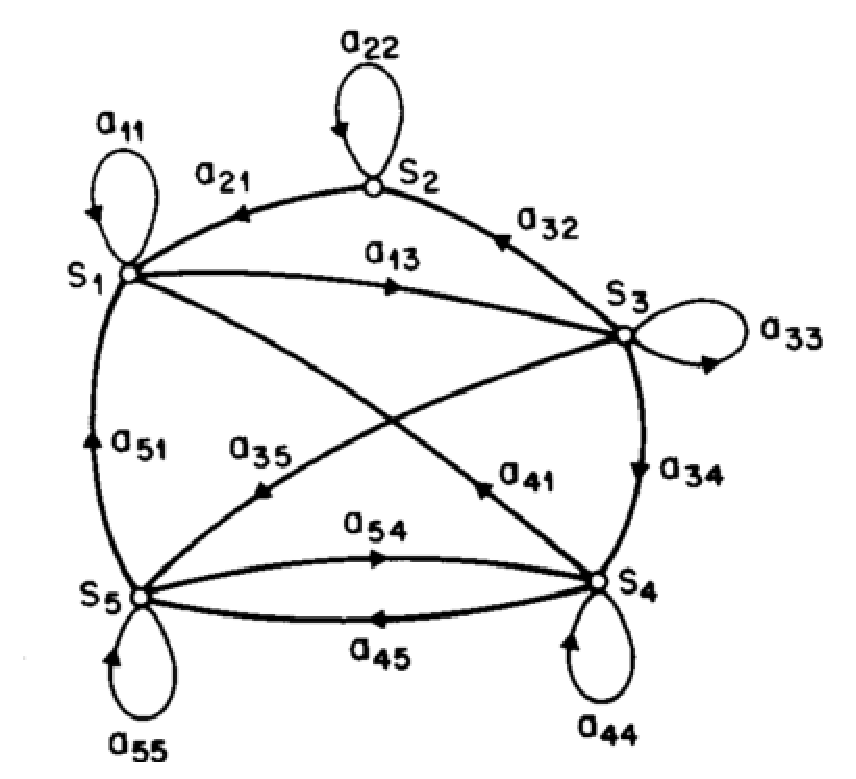
\includegraphics[width=.6\linewidth]{8_29_HMM_chain}\\
  \caption{A Markov chain with 5 states}\label{fig:chain}
\end{figure}

In the discrete Markov processes (without hidden states), a system at any time is described as being in one of a set of distinct state (cf. Figure \ref{fig:chain}). A full probabilistic description of the above system would require specification of the current state, as well as all the predecessor states. For the special case of a discrete, first order, Markov chain, it is assumed that the probabilistic description only depends on the current state and its immediate predecessor. This stochastic process is also called an observable Markov model, since the output of the process is the set of states at each instant of time, where each state corresponds to a physical (observable) event.

HMMs extend the concept to include the case where the observation is a probabilistic function of the hidden states, i.e., the resulting model is a doubly embedded stochastic process with an underlying stochastic process that is not observable, but can only be observed through another set of stochastic processed that produce the observations.

It would be better to explain the concept with the following example. Suppose on the other side of the curtain a person is performing a coin tossing experiment. That person will not tell you anything about what he is doing exactly (he may be tossing 2 or 3 different coins with different biased coins); he will only tell you the result of each coin flip (the observation).

\begin{figure}[htbp]
  \centering
  \subfigure{
    \label{fig:topka} %% label for first subfigure
    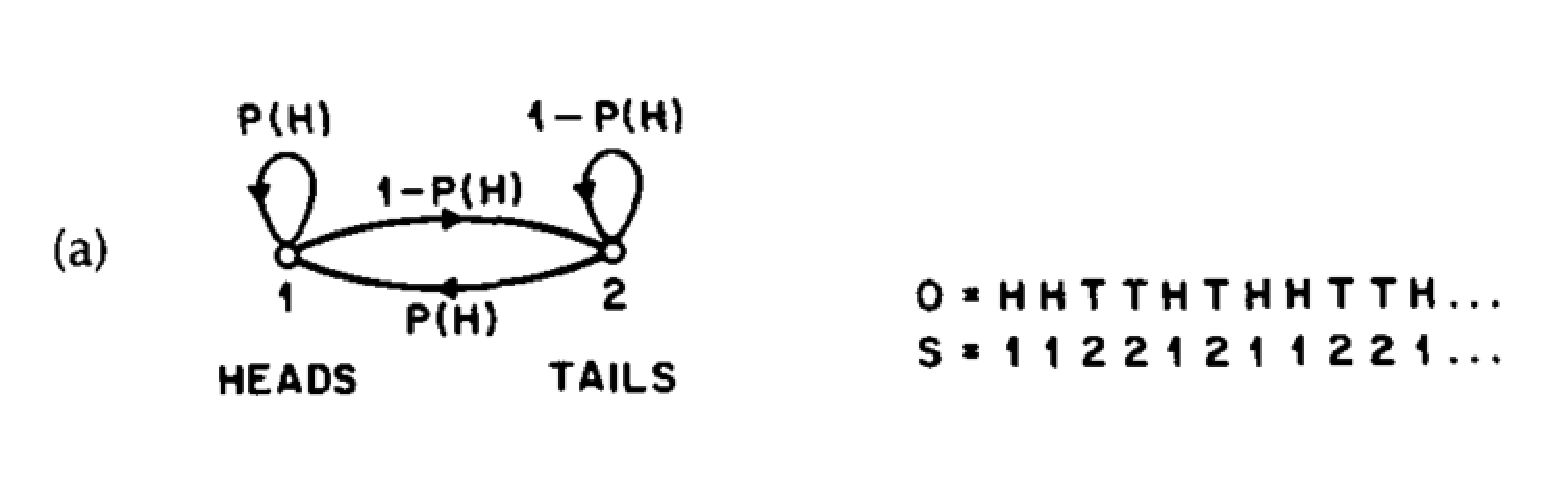
\includegraphics[width=2.2in]{8_29_HMM_coinA}}
  \subfigure{
    \label{fig:topkb} %% label for second subfigure
    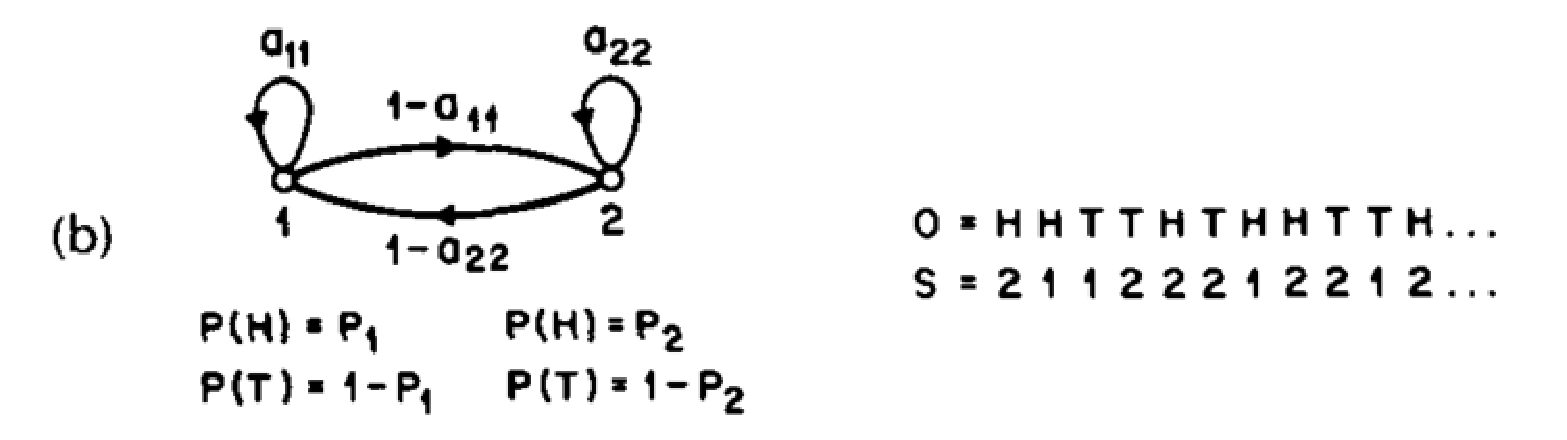
\includegraphics[width=2.2in]{8_29_HMM_coinB}}
  \subfigure{
    \label{fig:topkb} %% label for second subfigure
    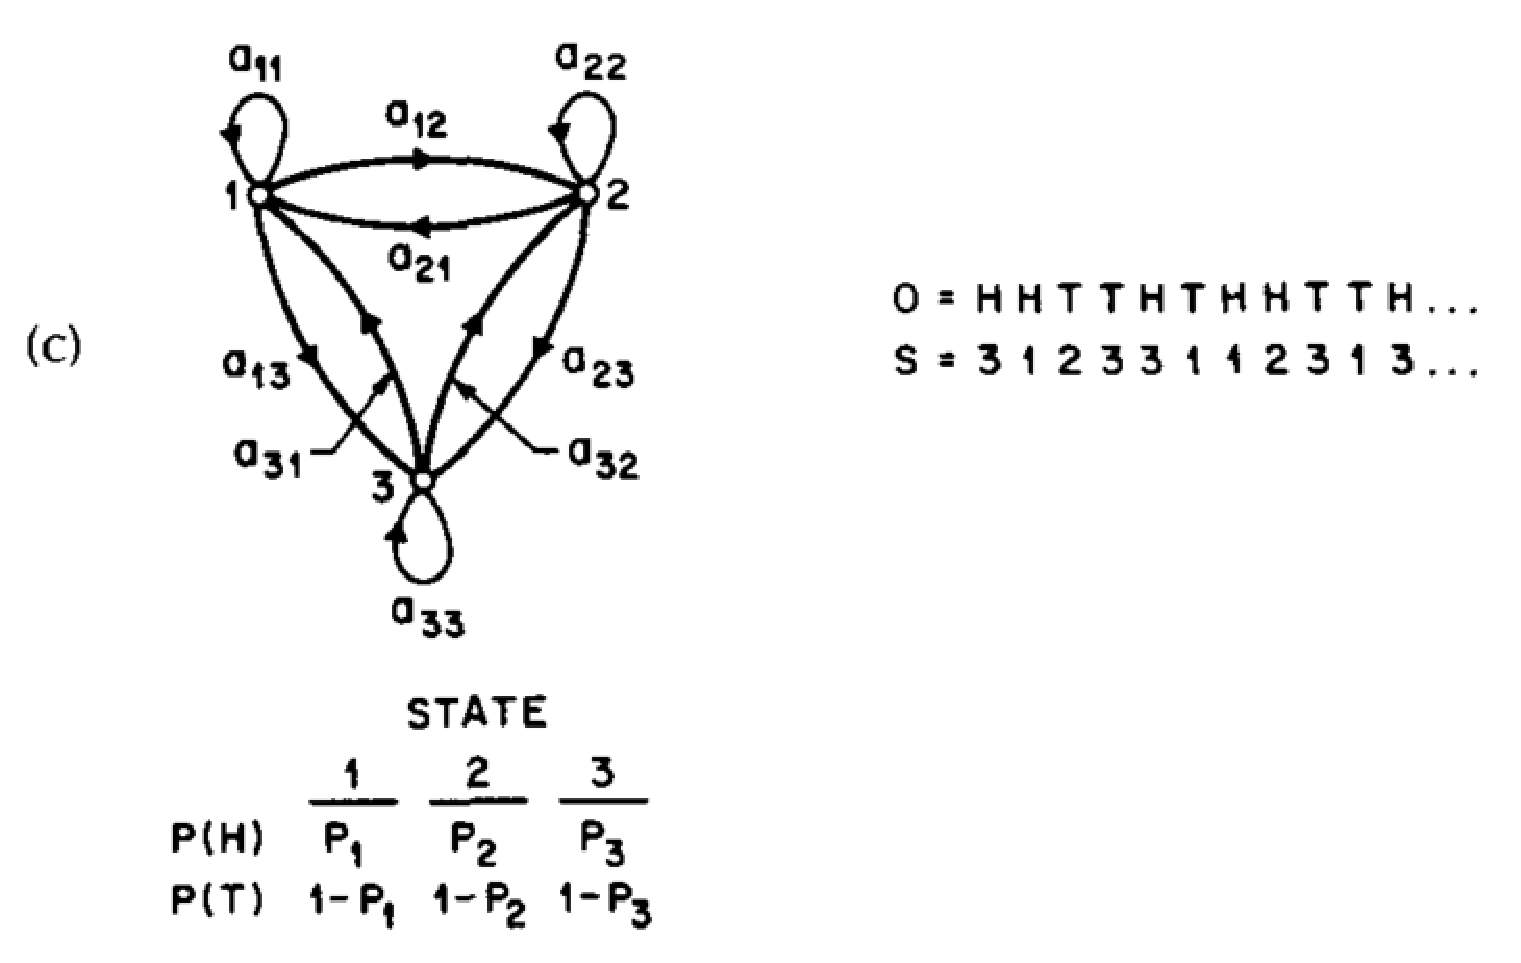
\includegraphics[width=2.2in]{8_29_HMM_coinC}}
  \caption{Three possible Markov models that can account for the results of hidden coin tossing experiments}\label{fig:coin}
\end{figure}

One possible choice would be to assume that only a single coin was being tossed. In this case the situation could be model with a 2-state (fully observable) model where each state corresponds to a side of the coin (cf. Figure \ref{fig:coin} (a)). We can also assume that two different biased coins were being tossed, and use the HMM in Figure \ref{fig:coin} (b) to describe this situation. Here each state corresponds to a different coin. Each state is characterized by a probability distribution of heads and tails, and transitions between states are characterized by a state transition matrix. We could further assume that there are 3 different coins, and model the system as a HMM with 3 hidden states (cf. Figure \ref{fig:coin} (c)).

An HMM is mathematically characterized by the following parameters: 1) $N$, the number of states in the model; 2) $M$, the number of distinct observation symbols; 3) The state transition probability distribution $A=\{a_{ij}\}$; 4) The observation symbol probability distribution in state $j$, $B = \{b_j(k)\}$; 5) The initial state distribution $\pi$. The paper uses the compact notation $\lambda = (A, B, \pi)$ to indicate the complete parameter set of the models.

There are three basic problems for HMMs: 1) How to efficiently compute $P(O| \lambda)$, the probability of the observation sequence given the model; 2) Given the observation sequence $O$ and the model $\lambda$, how to choose a corresponding state sequence $Q$ that is optimal; 3) How to adjust (or train) the parameters in $\lambda$ to maximize $P(O| \lambda)$.

The paper shows that all the three problems can be solved by the \emph{forward-backward procedure}. The basic idea of the forward-backward procedure is to apply the technique of dynamic programming. It introduces a forward variable $\alpha_t(i)$, which is probability of the partial observation sequence $O_1, ..., O_t$ (until time $t$) and state $S_i$ at time $t$. It shows how $\alpha_{t+1}(i)$ can be computed based on $\alpha_t(i)$ (the idea of dynamic programming). Similarly, a backward variable $\beta_t(i)$ is defined as the probability of the partial observation sequence from $t+1$ to the end. Finally, all the three problems can be solve by using the forward and backward variables.

In the remaining parts of the paper, it introduces various types of HMMs that have been previously studied (for example HMMs whose states are not fully connected). It also discusses the issues that arise in implementations, such as initial parameter estimates, model size, missing data, etc. Finally it describes some successful applications of HMMs in the field of speech recognizer. 
\subsection{Deep Neural Networks for Acoustic Modeling in Speech Recognition \cite{Hinton2012Deep}}

This paper provides an overview of the progress of acoustic modeling by \emph{deep neural networks (DNNs)}. It also presents the shared view of four research groups (groups at the University of Toronto, Microsoft Research, Google, and IBM Research) that have had recent successes in using this technique.

The goal of the acoustic modeling in this paper is to determine how well each state of a \emph{hidden Markov model (HMM)} fits a frame or a short window of frames of coefficients that represents the acoustic input $p(HMMstate | AcousticInput)$. So the produced acoustic model is combined with the classic HMM to form the final hybrid \emph{automatic speech recognition (ASR)} system.

In modern ASR systems, the acoustic input is typically represented by concatenating \emph{Mel-frequency cepstral coefficients (MFCCs)} or \emph{perceptual linear predictive coefficients (PLPs)}, computed from the raw waveform and their first- and second-order temporal differences. The preprocessing techniques are designed to discard the large amount of information in waveforms that is considered to be irrelevant for discrimination.

The DNN approach for acoustic modeling has two key stages. In the first stage, layers of feature detectors are initialized, one layer at a time, by fitting a stack of generative models. In the second stage, each generative model in the stack is used to initialize one layer of hidden units in a DNN. Finally the whole network is then discriminatively fine-tuned to predict the target HMM states.

The idea behind the first stage is generative pretraining: it finds a region of the weight-space that allows the discriminative fine-tuning to make rapid progress, and it also significantly reduces overfitting. The generative model in DNN approaches uses a set of parameters, $W$, to define the joint probability of a vector of observable variables $v$, and a vector of latent variables $h$, via an energy function $E$:
$$p(v,h; W) = \frac{1}{Z} e^{-E(v,h; W)}, Z = \sum_{v', h'} e^{-E(v', h'; W)}.$$
In the classic \emph{restricted Boltzmann machine (RBM)} which consists of a layer of stochastic binary visible units and a layer of stochastic binary hidden units, the energy function is defined to be:
$$E(v,h) = -\sum_{i \in  visible} a_i v_u - \sum_{j \in hidden} b_j h_j - \sum_{i,j} v_i h_i w_{ij},$$
where $v_i, h_j$ are the binary states of visible unit $i$ and hidden unit $j$, $a_i, b_j$ are their biases, and $w_{ij}$ is the weight between them. The training of a RBM can be achieved by the \emph{contrastive divergence (CD)} algorithm.

After training an RBM on the data, the inferred states of the hidden units can be used as data for training another RBM that learns to model the dependencies between the hidden units of the first RBM. This can be repeated many times to produce many layers of nonlinear feature detectors, which is called a \emph{deep believe network (DBN)}.

\begin{figure}[htbp]
  \centering
  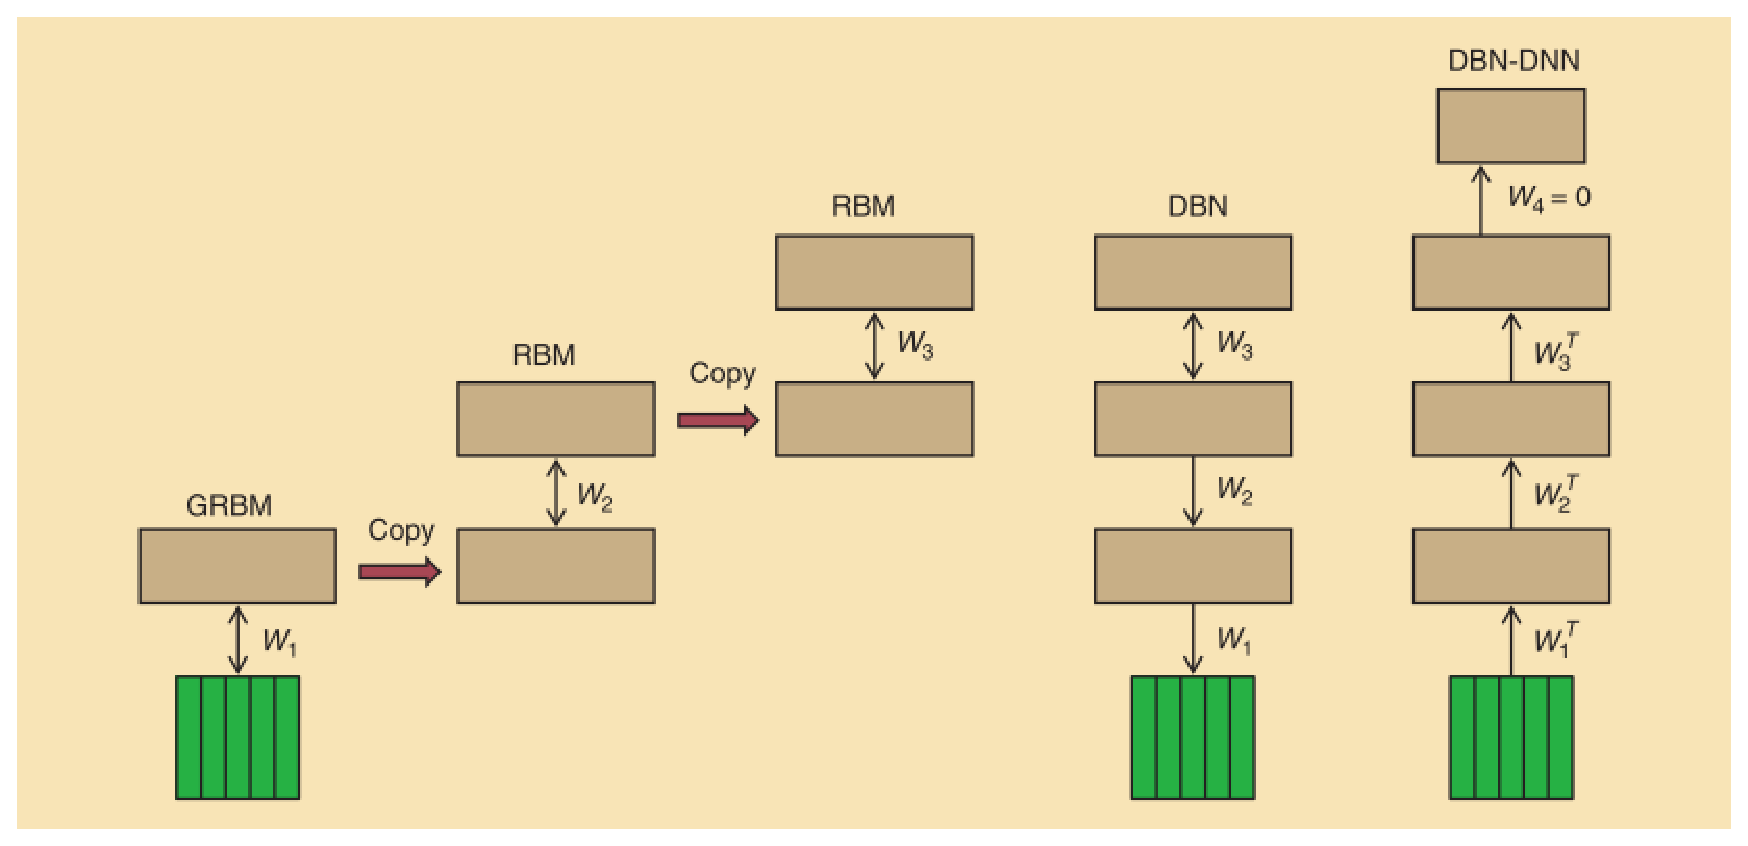
\includegraphics[width=.9\linewidth]{10_17_HMM_DNN}\\
  \caption{Illustration of the DNN training process}\label{fig:HMM_DNN}
\end{figure}

After learning a DBN by training a stack of RBMs, the generative weights in the reverse direction are used as the initialization of a feedforward DNN. It then adds a final softmax layer and trains the whole DNN discriminatively. The whole architecture is illustrated in Figure \ref{fig:HMM_DNN}: 1) A \emph{Gaussian RBM (GRBM)} is trained to model real-valued acoustic coefficients. Then the hidden states of the GRBM are used as data for training the next RBM. 2) This is repeated to create as many hidden layers as desired. 3) Finally, a pretrained DBN-DNN is created by adding a softmax output layer that predicts the hidden state of the HMM.

In the experimental study, the paper reports the results on the TIMIT benchmark and on several large-vocabulary speech recognition datasets. For example in the Bing-voice-search speech recognition task, the best DNN-HMM acoustic model achieves a sentence accuracy of 69.6\% on the test set, compared with 63.8\% for a strong HMM baseline method. 
\subsection{Speech Recognition With Deep Recurrent Neural Networks \cite{Graves2013Speech}}

End-to-end training methods such as \emph{Connectionist Temporal Classification (CTC)} make it possible to train RNNs for sequence labelling problems where the input-output alignment is unknown. However, RNN performance in speech recognition has so far been disappointing. This paper investigates deep recurrent neural networks on the ASR task, and shows that the method achieves a test set error of 17.7\% on the TIMIT phoneme recognition benchmark, which is the best recorded score.

The goal of this paper is to investigate whether RNNs could benefit from depth in space - that is, stacking multiple recurrent hidden layers on top of each other.

\begin{figure}[htbp]
  \centering
  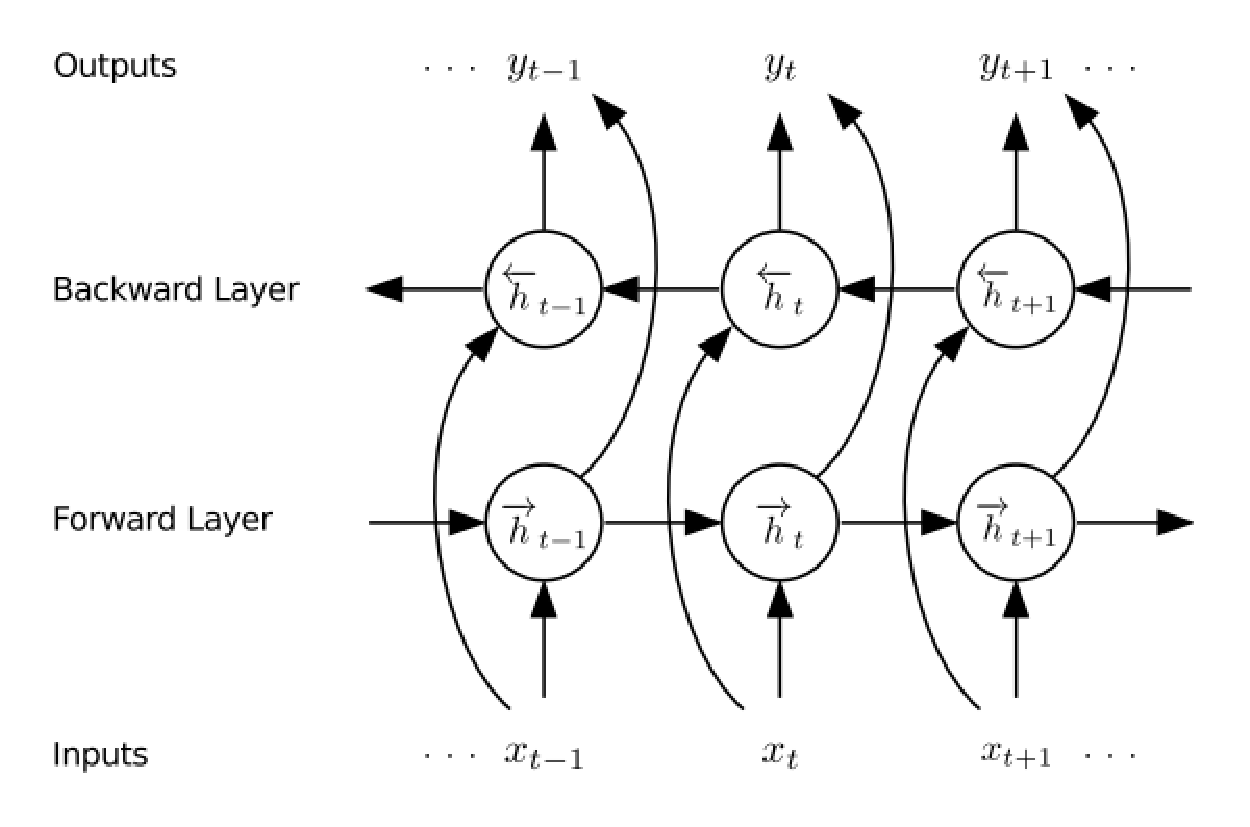
\includegraphics[width=.5\linewidth]{10_17_ASR_RNN}\\
  \caption{Bidirectional RNN}\label{fig:ASR_RNN}
\end{figure}

The concepts of RNN and \emph{long short-term memory (LSTM)} unit have been discussed in previous paper summaries. The basic architecture in this paper is based on the \emph{bidirectional RNNs (BRNNs)}. The basic idea of BRNN is to process the data in both directions (forward and backward) with two separate hidden layers. Figure \ref{fig:ASR_RNN} shows an example of a BRNN model that computes the forward hidden sequence $\stackrel{\rightarrow}{h}$, the backward hidden sequence $\stackrel{\leftarrow}{h}$, and the output sequence $y$. Combining BRNNs with LSTM gives \emph{bidirectional LSTM}.

In the RNN training, the RNNs map directly from acoustic to phonetic sequences. The paper presents two ways to define the output distribution and hence train the network.

The first method is called Connectionist Temporal Classification, which uses a softmax layer to define a separate output distribution $Pr(k|t)$ at every step $t$ along the input sequence. CTC then uses a \emph{forward-backward algorithm} to sum over all possible alignments and determine the normalised probability $Pr(z|x)$ of the target sequence.

The second method is based on the \emph{RNN transducer} technique, which combines a CTC-like network with a separate RNN that predicts each phoneme given the previous ones, thereby yielding a jointly trained acoustic and language model. The basic idea of RNN transducer is to determine a separate distribution $Pr(k | t, u)$ for every combination of input timestep $t$ and output timestep $u$. Specifically, $Pr(k | t, u)$ is defined by taking an `acoustic' distribution $Pr(k | t)$ from the CTC network, a `linguistic' distribution $Pr(k | u)$ from the prediction network, then multiplying them together and renormalising.

In the experimental study, the proposed model is evaluated on the TIMIT corpus. It is reported that the \emph{phoneme error rate (PER)} on the core test set is 17.7\%, which is the best result known to the authors.

Remark: I have also consider the possibility of applying RNNs on the ASR task. This paper shows that this is indeed a promising approach. Compared to the HMM-based or hybrid methods, the approach of this paper is simpler and more elegant - it can jointly train the acoustic and language models in an end-to-end fashion. However, this method is still not very mature, since the TIMIT benchmark is restricted in size. As mentioned by the authors, a possible future work is to extend the system to large vocabulary speech recognition. 
\subsection{Speech Recognition with Weighted Finite-State Transducers \cite{Mohri2000}}

This paper describes a general representation and algorithmic framework for speech recognition based on \emph{weighted finite-state transducers (WFST)}. These transducers provide a common and natural representation for major components of speech recognition systems, including \emph{hidden Markov models (HMMs)}, context-dependency models, pronunciation dictionaries, etc. The paper shows the application of the proposed method to large-vocabulary recognition task.

A \emph{finite-state transducer} is a finite automaton whose state transitions are labeled with both input and output symbols. Therefore, a path through the transducer encodes a mapping from an input symbol sequence, or string, to an output string. A weighted transducer puts weights on transitions in addition. In this paper, weights encode the probabilities that accumulates along the path.

\begin{figure}[h]
  \centering
  % Requires \usepackage{graphicx}
  \includegraphics[width=\linewidth]{11_21_WFST.png}\\
  \caption{Examples of weighted finite-state transducer}\label{fig:WFST}
\end{figure}

Figure \ref{fig:WFST} presents a toy language model and a toy pronunciation lexicon as WFSTs. In Figure \ref{fig:WFST}(b), the WFTS maps from phone strings to words in the lexicon, in this example `data' and `dew', with probabilities representing the likelihoods of alternative pronunciations. Similarly, HMM structures can be combined into a single transducer that preserves phone model identity.

The proposed method relies on a common set of weighted transducer operations to combine, optimize, search and prune them. The basic operations \emph{union}, \emph{concatenation}, and \emph{Kleene closure} operations combine transducers in parallel, in series, and with arbitrary repetition, respectively. There are three other key operations that are used in the speech applications:

1) \emph{Composition}: Composition is the transducer operation for combining different levels of representation. For example, a pronunciation lexicon can be composed with a word-level grammar to produce a phone-to-word transducer. In particular, the composition $T = T_1 \circ T_2$ has exactly one path mapping string $u$ to string $w$ for each pair of paths, the first in $T_1$ mapping $u$ to $v$ and the second in $T_2$ mapping $v$ to $w$.

2) \emph{Determinization}: In a deterministic transducer, each state has at most one transition with any given input label and there are no input $\epsilon$-labels. The key advantage of a deterministic transducer is its irredundancy: it contains at most one path matching any given input string, thereby reducing the time and space needed to process the string. The determinization algorithm transforms a non-deterministic WFST into an equivalent deterministic WFST.

3) \emph{Minimization}: Given a deterministic WFST, its size can be reduced by minimization, which can save both space and time. Let the given WFST be denoted as $A$. The minimization algorithm results in a WFST $B$ that is equivalent to $A$, and has the least number of states and the least number of transitions among all deterministic WFSTs equivalent to $A$.

Next we will see how to construct a single recognition transducer that maps from context-dependent phones to a string of words.

Consider the pronunciation lexicon $L$ in Figure \ref{fig:WFST}(b), and the grammar $G$ of Figure \ref{fig:WFST}(a). $L \circ G$ gives a transducer that maps from phones to word strings restricted to the grammar $G$. If we let $C$ represent a transducer from context-dependent phones to context-independent phones, then $C \circ (L \circ G)$ gives a transducer that maps from context-dependent phones (such as triphones) o word strings restricted to the grammar $G$. Finally, the transducer is optimized with determinization and minimization: $N = min(det(C \circ (L \circ G)))$.

In the following sections, the paper introduces the operation algorithms in further details, and reports the experimental results in the large-vocabulary speech recognition task. It is shown that the proposed method can greatly improve the efficiency and save space. 
\subsection{Efficient General Lattice Generation and Rescoring \cite{Ljolje1999}}

This paper describes a lattice generation method that produces high-quality lattices with less than 10\% increased computation over standard \emph{Viterbi} decoding. The proposed method is closely related to previous lattice generation methods, but applies to more general network topologies.

\begin{figure}[h]
  \centering
  % Requires \usepackage{graphicx}
  \includegraphics[width=.7\linewidth]{11_21_lattice.png}\\
  \caption{Example of a lattice}\label{fig:lattice}
\end{figure}

In this paper, a \emph{lattice} is defined to be a labeled, weighted, directed acyclic graph in which each complete path represents an alternative transcription hypothesis, weighted by its recognition score for a given utterance. However, it should be noted that there is no generally accepted single definition of lattice. Figure \ref{fig:lattice} shows an example of lattice (figure from Chapter 10 of Speech and Language Processing \cite{Jurafsky2006}).

In this paper, \emph{ASR networks} are represented as \emph{finite-state transducers}. These are labeled, weighted, directed graphs in which each arc $a$ has a source state $S(a)$, destination state $D(a)$, an input label $I(a)$, output label $O(a)$, and a weight $P(a)$. Here each input label is a context-dependent phone symbol, and each output label is a word. A complete path through such a transducer gives a legal sequence of words in the language model.

The recognition task can be characterized as finding a path $a = a_1,...,a_n$ that maximizes the joint probability of the acoustic and language models when applied to a given utterance:
$$\max_a P(\vec{x}[0, \tau], a) = \max_{a, t_1, ..., t_{n-1}}\prod_{i=1}^n P(\vec{x}[t_{i-1}, t_i] | I(a_i)) P(a_i).$$

The first factor represents the acoustic model likelihood for the context-dependent phone $I(a_i)$, and the second factor represents the language probability for that arc in the transducer $T$. Let $B(s)$ be the set of all paths in $T$ from the initial state to state $s$. Define
$$\alpha(s,t) = \max_{a \in B(s), t_1, ..., t_{k-1}} \prod_{i=1}^k P(\vec{x}[t_{i-1}, t_i] | a_i) P(a_i).$$
Then:
$$\max_{a} P(\vec{x}[0,t], a) = \max_{D(a)=s} p(a) [\max_{t' < t} P(\vec{x}[t',t]|I(a)) \alpha(S(a), t')].$$
In this way, the familia Viterbi recursion is factored into two nested loops: the outer loop considers each possible active arc $a$ ending in $s$, and the inner loop picks out the optimal start time $t'$.

The lattice generation algorithm consists of three main steps: 1) creates a context-dependent phone-to-word transducer lattice; 2) converts it to a word lattice; 3) prunes the lattice relative to the best scoring path.

In the first step, each state in lattice $L$ corresponds to a pair $(t,s)$ of a time frame in the recognition and a state from the transducer $T$. If during the Viterbi recursion, it has identified the optimal start time $t'$ for are $a$ ending in state $D(a)$ at time $t$, then a corresponding arc is added to $L$ from $(t', S(a))$ to $(t, D(a))$.

To convert the phone-to-word lattices to word lattices, it relies on the efficient implementations of the general finite-state operations. It deletes the input labels by the projection operator, and removes the $\epsilon$ arcs.

The final step is to prune the lattice relative to the best scoring path. The method is simple: the best score $\alpha(s)$ among paths from the initial state to state $s$ is found, as well as the best score $\beta(s)$ among paths from state $s$ to a final state. State for which $\alpha(s) + \beta(s) < \kappa \times \beta(s_0)$ are then pruned.

In the experimental section, it is shown that lattice generation requires typically less than 10\% additional computation time above one-best decoding. With the second pass, the proposed method is able to achieve a 3x real-time word error rate of 11.2\% on the Eval'95 test set. 
\subsection{Dialogue Act Modeling for Automatic Tagging and Recognition of Conversational Speech \cite{Stolcke2000}}

This paper describes a statistical approach for modeling \emph{dialogue acts (DAs)} on conversational speech, i.e., speech-act-like units such as \emph{Statement}, \emph{Question}, \emph{Backchannel}, etc. The proposed model detects and predicts dialogue acts based on lexical, collocational, and prosodic cues, as well as on the discourse coherence. It develops a probabilistic integration of speech recognition with dialogue modeling, to improve both speech recognition and dialogue act classification accuracy.

The goal of this paper is twofold: 1) presets a comprehensive framework for modeling and automatic classification of DAs, and proposes a framework that provides a mathematically principled way to condition the speech recognizer on conversation context through dialogue structure; 2) presents results obtained with this approach on a large, widely available corpus of spontaneous conversational speech.

This paper follows a recent standard for shallow discourse structure annotation, the \emph{Dialogue Act Markup in Several Layers (DAMSL)} tag set, which aims to provide a domain-independent framework for dialogue annotation.

The mathematical and computational framework used in the paper is the \emph{hidden Markov model (HMM)}. Given all available evidence $E$ about a conversation, the goal is to find the DA sequence $U$ that has the highest posterior probability $P(U|E)$ given that evidence.
$$U^* = \arg\max_U P(U|E) = \arg\max_U P(U) P(E|U).$$
Next we will discuss the prior probability $P(U)$, and the posterior probability $P(E|U)$ respectively.

In modelling the prior distribution $P(U)$, the paper assumes that the distribution is Markovian, i.e., each $U_i$ depends only on a fixed number $k$ of preceding DA labels:
$$P(U_i | U_1, ..., U_{i-1}) = P(U_i | U_{i-k}, ..., U_{i-1}).$$
The paper trains standard backoff N-gram models, using the frequency smoothing approach. The authors also tried several alternative approaches, but there was no significant improvement over the simple N-gram method.

The computation of $P(E|U)$ depends on the types of evidence use. The paper used the following three types of sources of evidence, either alone or in combination:
\begin{itemize}
\item{\textbf{Transcribed words}\\
$P(W|U)$, where $W$ refers to the true (hand-transcribed) words spoken in a conversation.
}
\item{\textbf{Recognized words}\\
A standard approach is to use the 1-best hypothesis. A more thorough approach is to compute $P(A|U)$ (where $A$ is the acoustics input) by decomposing it into an acoustic likelihood $P(A|W)$ and a word-based likelihood $P(W|U)$:
$$P(A|U) = \sum_W P(A|W) P(W|U).$$
}
\item{\textbf{Prosodic features}\\
$P(F|U)$, where $F$ are the features capturing various aspects of pitch, duration, energy, etc., of the speech signal. For the prosodic classifiers, the paper used CART-style decision trees. One example in the corpus was the distinction between backchannels and agreement. The prosodic tree trained on this task is shown in Figure \ref{fig:stolcke00-decision_tree}. The paper also tried to use neural network classifiers on this task, and tested
various network structures. However, there was no encouraging result.
\begin{figure}[h]
  \centering
  % Requires \usepackage{graphicx}
  \includegraphics[width=\linewidth]{stolcke00-decision_tree.png}\\
  \caption{Decision tree for the classification of backchannels and agreements.}\label{fig:stolcke00-decision_tree}
\end{figure}
}
\end{itemize}

The paper proposes a method to combine multiple knowledge source, by using the following approximation:
\begin{align*}
P(A_i, W_i, F_i | U_i) &= P(A_i, W_i | U_i) P(F_i | A_i, W_i, U_i)\\
                       &\approx P(A_i, W_i | U_i) P(F_i | U_i).
\end{align*}

The HMM representation allows using efficient dynamic programming algorithms to compute relevant aspects of the model, such as: 1) the most probable DA sequence (the \emph{Viterbi algorithm}); 2) the posterior probability of various DAs for a given utterance (the \emph{forward-backward algorithm}).

The paper considers ways to use DA modeling to enhance automatic speech recognition (ASR). The first method is called \emph{mixture-of posteriors}, which yields:
$$P(W_i | A_i, E) = \sum_{U_i} \frac{P(W_i | U_i) P(A_i | W_i)}{P(A_i | U_i)} P(U_i | E).$$
The second method, called \emph{mixture-of-LM}, results in:
$$P(W_i | A_i, E) \approx (\sum_{U_i} P(W_i | U_i) P(U_i|E)) \frac{P(A_i |W_i)}{P(A_i)}.$$

The experiments confirmed that DA modeling can improve word recognition accuracy quite substantially in principle, at least for certain DA types.But the skewed distribution of DAs limits the usefulness of the approach on the Switchboard corpus. The paper suggests that the benefits of DA modeling might be more pronounced on corpora with more even DA distribution, which is typically the case for task-oriented dialogues.

\subsection{Maximum Likelihood Linear Regression for Speaker Adaption of Continuous Density Hidden Markov Models \cite{Leggetter1995}}

Adaption techniques fall into two main categories - speaker normalization in which the input speech is normalized to match the speaker that the system is trained to model, and model adaptation techniques in which the parameters of the model set are adjusted to improved the modelling of the new speaker. This paper proposes a model adaptation technique which uses a set of regression-based transforms to tune the hidden Markov model (HMM) mean parameters to the new speaker.

The basic idea of the maximum likelihood linear regression (MLLR) method is to calculate the transformation matrices to maximize the likelihood of the adaptation data, and can be implemented using the forward-backward algorithm. By tying the transformations among a number of distributions, adaptation can be performed for distributions which are not represented in the training data.

Consider a continuous density HMM system with Gaussian output distribution. A particular distribution, $s$ is characterized by a mean vector, $\mu_s$, and a covariance matrix $C_s$. Given a parameterized speech frame vector $o$, the probability density of the vector is
$$b_s(o) = \frac{1}{(2\pi)^{n/2} |C_s|^{1/2}} e^{-\frac{1}{2(o - \mu_s)'G_s^{-1}(o-\mu_s)}}.$$

The adaptation of the mean vector is achieved by applying a transformation matrix $W_s$ to the extended mean vector $\xi_s$ to obtain an adapted mean vector $\hat{\mu_s}$: $\hat{\mu_s} = W_s \xi_s$. Here $\xi_s$ is defined as $\xi_s = [\omega, \mu_1, ..., \mu_n]'$, where $\omega$ is the offset term for the regression. For distribution $s$, the probability density function for the adapted system becomes
$$b_s(o) = \frac{1}{(2\pi)^{n/2} |C_s|^{1/2}} e^{-\frac{1}{2(o - W_s \xi_s)'G_s^{-1}(o-W_s \xi_s)}}.$$

A more general approach is that the same transformation matrix is used for several distributions. The transformation is estimated using data from all the associated tied distributions, so if some of the distributions are not observed in the adaptation data, a transformation may still be applied. The degree of transformation tying is determined by the amount of adaptation data available. For the case of small amounts of adaptation data a global transformation may be used.

The following sections of this paper describes the method in further details, specifically proposes how to use to forward-backward algorithm to train the transformation matrix.

In the experimental study, it is shown that with the proposed method adaptation can be performed using as little as 11s of adaptation data, and that as more data is used the adaptation performance improves. For example, using 40 adaptation utterances, a 37\% reduction in error from the speaker-independent system was achieved with supervised adaptation and a 32\% reduction in unsupervised mode. 

